
%(BEGIN_QUESTION)
% Copyright 2012, Tony R. Kuphaldt, released under the Creative Commons Attribution License (v 1.0)
% This means you may do almost anything with this work of mine, so long as you give me proper credit

Anta at en automatikker ønsker å bruke en loop kalibrator til å simulereet 4-20mA signal til en regulator. Han kobler den opp slik bildet viser. 

$$\includegraphics[width=15.5cm]{i00011x01.eps}$$

Forklar hvorfor det ikke går å koble en loop kalibrator på denne måten, og hva som vil skje om han prøver på det. Tilslutt skal du vise den korrekte måten en kan bruke en loop kalibrator for å simulere en transmitter. 

\vfil

\underbar{file i00011}
\eject
%(END_QUESTION)





%(BEGIN_ANSWER)

This is a graded question -- no answers or hints given!

%(END_ANSWER)





%(BEGIN_NOTES)

The problem here is that the transmitter is still in the circuit, passing its own current.  The 9 mA passed by the loop calibrator in ``simulate'' mode will become {\it added} to the transmitter's current to form a larger total current seen at the 250 ohm resistor.

The proper way to use the loop calibrator is like this:

$$\includegraphics[width=15.5cm]{i00011x02.eps}$$

%INDEX% Electronics review: 4-20 mA loop calibrator (test equipment)

%(END_NOTES)


